\documentclass{bachelor_report}

% Додаткові пакети вносіть у цей файл
\usepackage{euscript}

\usepackage{fontspec}

\setromanfont{PTSerif}[
    Path=./fonts/,
    Extension = .ttf,
    UprightFont = *-Regular,
    BoldFont = *-Bold,
    ItalicFont = *-Italic,
    BoldItalicFont = *-BoldItalic,
]


% Додаткові визначення та перевизначення команд вносіть у цей файл
\let\oldemptyset\emptyset
\let\emptyset\varnothing
\let\geq\geqslant
\let\leq\leqslant

\NewDocumentCommand{\set}{o m}{%
  % <code>
  \IfNoValueTF{#1}
    {\{#2\}}
    {\{#1 \mid #2\}}%
  % <code>
}




% Відомості про автора роботи
\newcommand{\reportAuthor}
{Житкевич Іван Олександрович}
\newcommand{\reportAuthorGroup}
{ФІ-91}
\newcommand{\reportTitle}
{Латинські квадрати. Завершення часткових латинських квадратів.}

\newcommand{\supervisorFio}
{Прізвище І.П.}
\newcommand{\supervisorRegalia}
{степінь, звання}


% Починаємо верстку документа
\begin{document}

\setfontsize{14}

% Створюємо титульну сторінку
% Титульный лист
\thispagestyle{empty}

\begin{center}
НАЦІОНАЛЬНИЙ ТЕХНІЧНИЙ УНІВЕРСИТЕТ УКРАЇНИ \par
<<КИЇВСЬКИЙ ПОЛІТЕХНІЧНИЙ ІНСТИТУТ ім. Ігоря СІКОРСЬКОГО>>\par
ФІЗИКО-ТЕХНІЧНИЙ ІНСТИТУТ\par

\vspace{40mm}
{\huge Есе на тему \par}

\huge\MakeUppercase{\textbf{\reportTitle}} \par
\end{center}

\vspace{40mm}
\begin{flushright}
Виконав студент

групи \reportAuthorGroup

\reportAuthor

\vspace{20mm}
% Науковий керівник:

% \supervisorRegalia

% \supervisorFio

\end{flushright}

\vspace{20mm}
\begin{center}
{Київ~--- 2020}
\end{center}

\newpage


%% Створюємо зміст    % -- розкоментуйте, якщо зміст вам потрібен
%\pagenumbering{gobble}
%\tableofcontents
%\cleardoublepage
%\pagenumbering{arabic}

\setcounter{page}{2}    %!!! -- продумати, як автоматизувати номер сторінки

%% Якщо ви використовуєте зміст, то прослідкуйте, щоб номер сторінки 
%% співпадав із справжнім!

% Створюємо перелік умовних позначень, скорочень і термінів
% Якщо цей розділ вам не потрібен, просто закоментуйте два наступних рядка
% \shortings
% ФТІ --- Фізико-технічний інститут

$\xor$ --- операція побітового додавання  %зауважте, що використовується перевизначена операція \xor


(Якщо ви не використовуєте перелік умовних позначень, просто приберіть 
даний розділ.)


% Створюємо вступ
\intro
%!TEX root = ../thesis.tex
% створюємо вступ
У вступі ви коротенько (приблизно на сторінку) повинні окреслити 
актуальність вашого дослідження, тематику та проблематику, а також 
окреслити, яке саме завдання ви розв'язували при виконанні даного звіту. 
Без чіткої виразної постановки задачі дослідження, яка буде 
розв'язуватись на подальших сторінках, ніхто не зрозуміє, що тут 
відбувається, і до вас виникне багато, дуже багато запитань. Воно вам 
треба?

Зрозуміло, що звіт зазвичай присвячено огляду опублікованих результатів 
(якщо мова йде про грудневий звіт) або конкретно вашим результатам (якщо 
мова йде про переддипломну практику), однак це занадто загально. У вступі 
ви повинні окреслити, який саме огляд ви робите (наприклад: \emph{<<У даному звіті 
викладено результати новітніх методів сепулєнія на основі пост-квантово 
стійких сепулярізаторів, популярність яких була зумовлена...>>} і~т.д.), 
або які саме наукові результати збираєтесь одержати згідно ваших 
дослідницьких задач (які в майбутньому стануть задачами вашого 
бакалаврського чи магістерського диплому).

% Додаємо глави
% Якщо ваша робота містить менше або більше глав - модифікуйте наступні 
% рядки відповідним чином
\chapter{Огляд та затягнутий вступ}

\section{Історія}

Ідея латинських квадратів породжується якнайменше 300 років тому у монограмі \emph{Koo-Soo-Ryak}, яку написав Choi Seok-Jeong (1646-1715). 
Він використовував ортогональні латинські квадрати 9 порядку для побудови магічних квадратів. У своїх нотатках він зауважив, що не міг знайти ортогональні латинські квадрати 10 порядку.

Але це не перша поява латинських квадратів. Існують амулети латинських квадратів середньовічного Ісламу, магічний квадрат аль-Буні. Вони доказують, що люди того часу знали мінімум 2 ортогональні латинські квадрати розміру $4\times 4$.

Тобто все ж невідоме точне походження латинських квадратів.

У 1776 році Ойлер презентував роботу \emph{De Quadratis Magicis} Академії Наук в Петербурзі. Там він показав побудову магічних квадратів порядку 3, 4, 5 з ортогональних квадратів. Також він продемонстрував проблему щодо магічного квадрату порядку 6, яка відома як \emph{Euler's 36 Officers Problem}. Надалі Ейлер припускав, що не існує таких рішень для порядку 6, та навіть пішов далі --- не існує ортогональних латинських квадратів порядку $n \equiv 2 (\operatorname{mod} 4)$.

Але його останнє припущення було спростовано 1958 року Раджом Бозе та Шарадчандром Шрікханде, які побудували два ортогональні латинські квадрати 22 порядку. Далі у 1960 році вони дізналися, що два ортогональні латинські квадрати порядку $n$ існують для всіх $n \equiv 2(\operatorname{mod} 4)$, окрім 2 та 6.


\section{Латинські квадрати та часткові латинські квадрати}

\begin{definition}
    Латинський квадрат порядку $n$ це матриця $L$ розміру $n \times n$ з елементами із множини $\set{1, \dots, n}$, де кожен елемент зустрічається у кожному рядку та колонці лише один раз.
\end{definition}

\begin{align*}
    L_{4,0} = \begin{bmatrix}
        0 & 1 & 2 & 3 \\
        3 & 0 & 1 & 2 \\
        2 & 3 & 0 & 1 \\
        1 & 2 & 3 & 0
    \end{bmatrix} 
    \;\; & \;\;
    L_{3,0} = \begin{bmatrix}
        1 & 0 & 2 \\
        0 & 2 & 1 \\
        2 & 1 & 0
    \end{bmatrix}
\end{align*}

Одне з найбільших досліджень латинських квадратів стосується часткових латинських квадратів.

\begin{definition}
    Частковий латинський квадрат порядку $n$ це матриця $P$ розміру $n \times n$, де кожне місце або пусте, або містить елемент із множини $\set{1, \dots, n}$ з умовою, що кожний елемент зустрічається у кожному рядку (колонці) лише один раз.
\end{definition}

Одне з важливих досліджень латинських квадратів розпочав Маршалл Голл та Герберт Джон Райзер. Воно стосується характеризації часткових латинських квадратів. Вже останні можуть бути доповнені до латинських квадратів без додавання рядків, колонок чи елементів. 

\begin{figure}[ht]
    \begin{subfigure}[b]{0.5\textwidth}
        \centering
        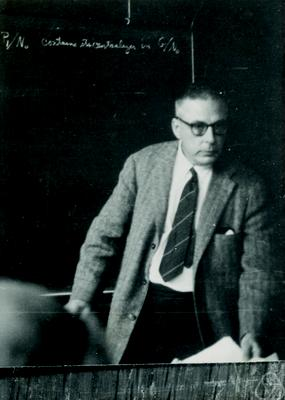
\includegraphics[scale=0.3]{Images/Marshall_Hall.jpg}
        \caption*{Маршалл Голл}
    \end{subfigure}
    \begin{subfigure}[b]{0.5\textwidth}
        \centering
        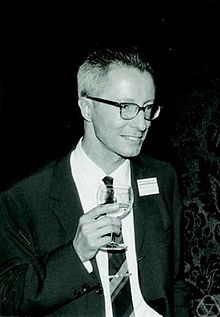
\includegraphics[scale=0.4]{Images/Herbert_Ryser.jpg}
        \caption*{Герберт Райзер}
    \end{subfigure}
\end{figure}


\chapter{(Назва другого розділу)}
\label{chap:theory}

До другого розділу також краще написати малесенький вступ. Зокрема, це 
збільшує загальний об'єм роботи та покращує її читабельність.

Якщо вам не потрібен другий розділ, то просто закоментуйте відповідний 
рядок у головному файлі.

\section{(Якийсь підрозділ)}

У другому розділі необхідно наводити розв'язання поставленої перед вами 
задачі у теоретичному або аналітичному сенсі (хоча, звісно, все залежить 
від того, яка саме задача перед вами поставлена).

Для подання матеріалів можна використовувати таблиці (наприклад, 
Таблицю \ref{tab_weight}).

    \begin{table}[ht]
    \setfontsize{14pt}
    \caption{Расчет весомости параметров ПП}
    \label{tab_weight}
    \centering
        \begin{tabular}{|c|c|c|c|c|c|c|c|c|}
        \hline \multirow{2}{*}{Параметр $x_i$} & \multicolumn{4}{c|}{Параметр $x_j$} & 
            \multicolumn{2}{c|}{Первый шаг} & \multicolumn{2}{c|}{Второй шаг} \\
        \cline{2-9} & $X_1$ & $X_2$ & $X_3$ & $X_4$ & $w_i$ & 
            ${K_\text{в}}_i$ & $w_i$ & ${K_\text{в}}_i$ \\
        \hline $X_1$ & 1 & 1 & 1.5 & 1.5 & 5 & 0.31 & 19 & 0.32 \\
        \hline $X_2$ & 1 & 1 & 1.5 & 1.5 & 5 & 0.31 & 19 & 0.32 \\
        \hline $X_3$ & 0.5 & 0.5 & 1 & 0.5 & 2.5 & 0.16 & 9.25 & 0.16 \\
        \hline $X_4$ & 0.5 & 0.5 & 1.5 & 1 & 3.5 & 0.22 & 12.25 & 0.20 \\
        \hline \multicolumn{5}{|c|}{Итого:} & 16 & 1 & 59.5 & 1 \\
        \hline
        \end{tabular}
    \end{table}

Бажано, щоб кожен пункт завдань, окреслених у вступі, відповідав певному 
розділу або підрозділу у дипломній роботі.

\begin{theorem}
Нумерація у наступних розділах також відбувається автоматично
\end{theorem}

\section{(Якийсь наступний підрозділ з дуже-дуже довгою назвою, загальна кількість слів в якій, однак, не повинна перевищувати 12 слів)}

Для подання матеріалів також дуже зручними є рисунки (наприклад, рисунки 
\ref{fig_sudak} або \ref{fig_pacman}).

\begin{figure}[ht]
\centering
    \begin{subfigure}[b]{0.5\textwidth}    
        
\includegraphics[scale=0.3]{Images/Sudak.png}
        \caption{}
        % обратите внимание на знак % после \end{subfigure} и 
        % отсутствие пустых строк и разделителей после \end{subfigure}
        % -- это сливает в одну строку подфигуры
    \end{subfigure}%
    \begin{subfigure}[b]{0.5\textwidth}
        
\includegraphics[scale=0.3]{Images/Tudak.png}
        \caption{}
    \end{subfigure}
 
    \caption{Различные виды рыб: (a) судак, (б) тудак.}
    \label{fig_sudak}
\end{figure}

\begin{figure}[ht]
        \centering
        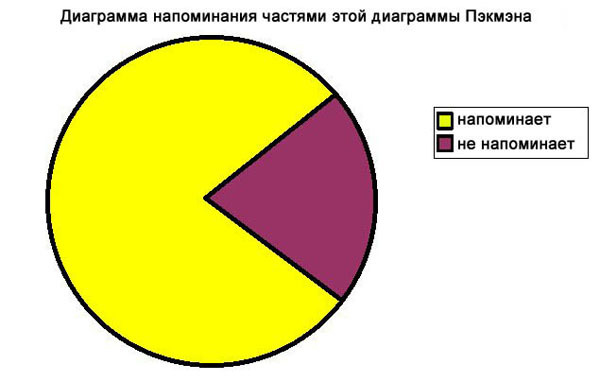
\includegraphics[scale=0.5]{Images/Pacman.jpg}
        \caption{Количество круговых диаграмм, похожих на Пэкмена}
        \label{fig_pacman}
\end{figure}


\chapconclude{\ref{chap:theory}}

Наприкінці розділу знову наводяться коротенькі підсумки.


% Створюємо висновки
\conclusions
У даній роботи ми розглянули питання складності доповнення часткових латинських квадратів, також згадали про застосування такої структури у криптографії.
Побудований латинський квадрат може бути використаний у створенні криптографічної системи.

Загалом, тема латинських квадратів є вузькою. Алгебраїчно, латинський квадрат це таблиця множень квазігрупи. Дослідження цього привели до застосувань у алгебрі, комбінаториці, теорії графів та інших розділів.


% Додаємо бібліографію
% Якщо ви володієте магією bibtex-у, використовуйте її та модифікуйте файл 
% з бібліографією відповідним чином
\begin{thebibliography}    
    \bibitem{colbourn82}
    Coulbourn, \textit{The Complexity of Completing Partial Latin Squares}, 22 April 1982, Department of Computational Science, University of Saskatchewan, Saskatoon. Saskatchewan, S7N 0 WO, Canada.

    \bibitem{padraic}
    Padraic Bartlett, \textit{3SAT and Latin Squares}, Department of Mathematics, University of California, Santa Barbara, 2014, <\url{http://web.math.ucsb.edu/~padraic/mathcamp_2014/np_and_ls/mc2014_np_and_ls_lecture4.pdf}>.

    \bibitem{schmidt}
    Nathan O. Schmidt, \textit{Latin Squares and their Applications to Cryptography}, December 2016.

    \bibitem{shao}
    Jia-yu Shao, Wan-di Wei, \textit{Note: A formula for the number of Latin squares}, 20 November 1990.

 
\end{thebibliography}


\end{document}
